\section{Uncertainty penalization}

The last classification approach explored differs substantially from its predecessors. In this new paradigm, the primary objective is no longer the implementation of an "I don't know" behavior; instead, the focus shifts towards consistently generating predictions at all the times. This approach can be useful in contexts where the application is non-critical, placing a greater importance on obtaining an output, even if erroneous. This is due the fact that a system interruption could potentially result in higher economic losses than a wrong prediction.

The idea to achieve this objective involves assigning penalties to the individual components of the predicted vector based on their associated uncertainties. During the classification process, the class with the highest probability prediction is chosen. By introducing penalization that accounts for the probabilities uncertainty, it could be feasible to redistribute information. For example, when the two highest probabilities exhibit close values, such as $0.30$ and $0.31$, the conventional prediction would favor the second class. However, it's possible that the uncertainty linked to the second value is higher. Through this penalization mechanism, the classification outcome could potentially shift to favor the first class instead.

The experiments were done with both the aleatoric and epistemic uncertainties. Let be $s_i$ the uncertainty of the probability $p_i$, the penalized value is $p_i^* = \frac{p_i}{1 + s_i \cdot \alpha}$, where $\alpha$ is intended to be the confidence level, accentuating the significance of the penalization. The $1$ in the denominator is added to avoid a division by $0$ in case of $s_i$ very close to $0$.

In \Fig~\ref{fig:aleat_penalization} are shown the results when the aleatoric uncertainty is employed. It is evident that there are no improvements for any confidence level. The accuracy stays around the nominal value. The observed fluctuations are due to the inherent stochastic nature of the network.It is worth noting that the observed changes remain in the vicinity of approximately $0.2\%$, which is not a significant impact. The same behavior is observed when using the epistemic uncertainty, as illustrated in \Fig~\ref{fig:epis_penalization}. This results demonstrate that with a BNN it is not possible to gain more information from the uncertainty, it is only possible to determine when the network is not sure and therefore it does not know what to output.

These results shows that with a BNN is not able to extract additional information from uncertainty. Instead, it can only be used as an indicator of the network inability to produce confident outputs.

\begin{figure}[h]
	\centering
	\begin{subfigure}{.5\textwidth}
		\centering
		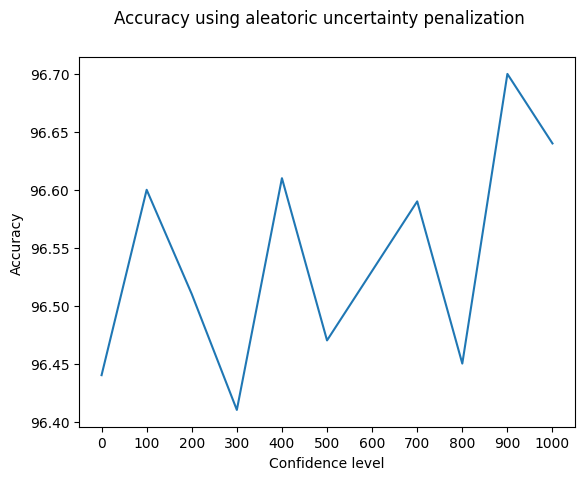
\includegraphics[width=0.8\linewidth]{ImageFiles/ClassifUncer/aleat_penalization}
		\caption{Accuracy trend with aleatoric uncertainty penalization}
		\label{fig:aleat_penalization}
	\end{subfigure}%
	\begin{subfigure}{.5\textwidth}
		\centering
		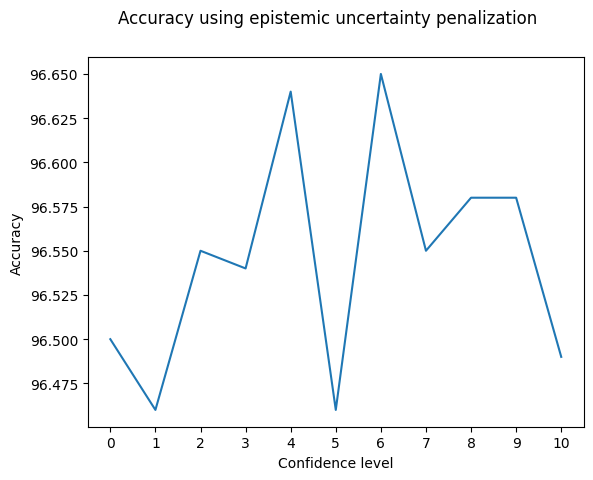
\includegraphics[width=0.8\linewidth]{ImageFiles/ClassifUncer/epis_penalization}
		\caption{Accuracy trend with epistemic uncertainty penalization}
		\label{fig:epis_penalization}
	\end{subfigure}
	\caption{Performances of the BNN with uncertainty penalization}
	\label{fig:penalization_class}
\end{figure}

Therefore, it is possible to assess that this approach does not yield to any performance improvement, and as a result, it will be excluded from the subsequent analysis.